\documentclass[a4paper,10pt]{jsarticle}

% レイアウト
\setlength{\textwidth}{\fullwidth}
\setlength{\textheight}{39\baselineskip}
\addtolength{\textheight}{\topskip}
\setlength{\voffset}{-0.5in}
\setlength{\headsep}{0.3in}
\pagestyle{myheadings}

% パッケージ
\usepackage[dvipdfmx]{graphicx}
\usepackage{amsmath,amssymb,epsfig}
\usepackage{bm}
\usepackage{ascmac}
\usepackage{pifont}
\usepackage{multirow}
\usepackage{enumerate}
\usepackage{cases}
\usepackage{type1cm}
\usepackage{cancel}
\usepackage{url}
\usepackage[dvipdfmx]{color}
\usepackage{listings,jlisting}
% 大きな中括弧
\usepackage{cases}

% 定義
\DeclareMathOperator*{\argmin}{arg\,min}
\DeclareMathOperator*{\argmax}{arg\,max}
% \def\vec#1{\mbox{\boldmath$#1$}}
\def\R{{\Bbb R}}

% カウンタの設定
\setcounter{section}{0}
\setcounter{subsection}{0}
\setcounter{subsubsection}{0}
\setcounter{equation}{0}

% キャプションの図をFigに変更
\renewcommand{\figurename}{Fig.}
\renewcommand{\tablename}{Tab.}

% 式番号を式(章番号.番号)に
% \makeatletter
% \renewcommand{\theequation}{\arabic{section}.\arabic{equation}}
% \@addtoreset{equation}{section}
% \makeatother

% プログラムに色をつける
\usepackage{color}

\definecolor{codegreen}{rgb}{0,0.6,0}
\definecolor{codegray}{rgb}{0.5,0.5,0.5}
\definecolor{codepurple}{rgb}{0.58,0,0.82}
\definecolor{backcolour}{rgb}{0.95,0.95,0.92}

\lstdefinestyle{mystyle}{
    backgroundcolor=\color{backcolour},
    commentstyle=\color{codegreen},
    keywordstyle=\color{magenta},
    numberstyle=\tiny\color{codegray},
    stringstyle=\color{codepurple},
    basicstyle=\footnotesize,
    breakatwhitespace=false,
    breaklines=true,
    captionpos=b,
    keepspaces=true,
    numbers=left,
    numbersep=5pt,
    showspaces=false,
    showstringspaces=false,
    showtabs=false,
    tabsize=2
}

\lstset{style=mystyle}

% % ドキュメントの開始
\begin{document}

\section{実行方法}
\subsection{動作環境}
LinuxのディストリビューションのひとつであるUbuntuで動作を確認している.
Ubuntuで動作させるための必要なアプリケーションは以下の通りである.

\begin{lstlisting}[basicstyle=\ttfamily\footnotesize, language=Bash, frame=single, firstnumber=1, numbers=left, breaklines=true]
sudo apt-get install build-essential
sudo apt-get install cmake
sudo apt-get install gnuplot
\end{lstlisting}

コンパイル時に必要なビルドシステムはbuild-essentialとcmakeが必要である.
ベジエ曲線や曲面をプロットするためにgnuplotを用いている.

Visual Studioでのコンパイルも可能であるが,その場合Struct.hの最初の記述を変更する.

\begin{lstlisting}[basicstyle=\ttfamily\footnotesize, language=C, frame=single, firstnumber=4, numbers=left, breaklines=true]
#define _CRT_SECURE_NO_DEPRECATE
#include <stdio.h>
#include <stdlib.h>
#define _USE_MATH_DEFINES
#include <math.h>
\end{lstlisting}

\subsection{ファイル構造}
このzipの中のファイル構造を示す.

\begin{lstlisting}[basicstyle=\ttfamily\footnotesize, language=Bash, frame=single, firstnumber=1, numbers=left, breaklines=true]
.
├── CMakeLists.txt
├── Struct.h
├── document
│  └── document.pdf
├── kadai.h
├── kadai1A.cpp
├── kadai1A.h
├── kadai3.cpp
├── kadai3.h
├── main.cpp
└── plot
    ├── InputPoint.dat
    ├── plot.plt
    ├── point.dat
    └── surfacedata.dat
\end{lstlisting}
InputPoint.datが課題3の制御点データファイルである.plot.pltがgnuplotでプロットするためのファイルで,point.datが制御点プロット用データ,surfacedata.datが曲面を表すプロット用データである.

\begin{lstlisting}[basicstyle=\ttfamily\footnotesize, language=Bash, frame=single, firstnumber=1, numbers=left, breaklines=true]
cd plot
gnuplot
load "plot.plt"
\end{lstlisting}

\subsection{コンパイル方法と実行方法}

\begin{lstlisting}[basicstyle=\ttfamily\footnotesize, language=Bash, frame=single, firstnumber=1, numbers=left, breaklines=true]
mkdir build
cd build
cmake ..
make
./実行ファイル名
\end{lstlisting}

\section{計算方法}
\subsection{ベジエ曲線}
ベジエ曲線上の点$q^3(t)$は下の式によって定義される.
\begin{equation}
\label{eq:a}
  q^3(t) = \left[
    \begin{array}{cccc}
      \vec{P_0} & \vec{P_1} & \vec{P_2} & \vec{P_3} \\
    \end{array}
  \right]\cdot M_B \cdot
  \left[
    \begin{array}{c}
      t^0\\
      t^1\\
      t^2\\
      t^3\\
    \end{array}
  \right]
\end{equation}

\begin{equation}
\label{eq:b}
  M_B =
  \left[
    \begin{array}{cccc}
      1 & -3 & 3 & -1 \\
      0 & 3 & -6 & 3\\
      0 & 0 & 3 & -3\\
      0 & 0 & 0 & 1\\
    \end{array}
  \right]
\end{equation}

制御点$\vec{P_0}$,$\vec{P_1}$,$\vec{P_2}$, $\vec{P_3}$は$\vec{P}=\left[
    \begin{array}{c}
      x\\
      y\\
      z\\
      1\\
    \end{array}
  \right]$
のように定義される.また$t$は$0\leqq t \leqq 1$である実数である.

\subsection{ベジエ曲面}
ベジエ曲面上の点は下の式で表される.
制御点行列$P$の成分である$P_{ij}$はそれぞれ$[x,\ y,\ z]$の成分を持っているので,計算をする際注意する.
\begin{equation}
\label{eq:c}
  q^3(u,\ v) = \left[
    \begin{array}{cccc}
      u^0 & u^1 & u^2 & u^3 \\
    \end{array}
  \right]\cdot M_B^{\mathrm{T}}P M_B \cdot
  \left[
    \begin{array}{c}
      v^0\\
      v^1\\
      v^2\\
      v^3\\
    \end{array}
  \right]
\end{equation}

\begin{equation}
\label{eq:d}
  P =
  \left[
    \begin{array}{cccc}
     P_{00} & P_{01} & P_{02} & P_{03} \\
     P_{10} & P_{11} & P_{12} & P_{13}\\
     P_{20} & P_{21} & P_{22} & P_{23}\\
     P_{30} & P_{31} & P_{32} & P_{33}\\
    \end{array}
  \right]
\end{equation}

\section{実行結果}
パラメータ値ごとに曲面上の点を求め,3次ベジエ曲面を作成した結果をFig.~\ref{fig:パラメータ値ごとに曲面上の点}に示す.
そして$\{P_{01},\ P_{01},\ P_{02},\ P_{03}\}$$\{P_{10},\ P_{11},\ P_{12},\ P_{13}\}$$\{P_{20},\ P_{21},\ P_{22},\ P_{23}\}$$\{P_{30},\ P_{31},\ P_{32},\ P_{33}\}$としたときの曲線上の点をプロットしたときの結果をFig.~\ref{fig:曲線上の点}に示す.
最後にベジエ曲線,曲面を同時にプロットしたときの様子をFig.~\ref{fig:ベジエ曲面と曲線を同時にプロットしたときの様子}に示す.

\begin{figure}[b]
 \begin{minipage}{0.5\hsize}
  \begin{center}
   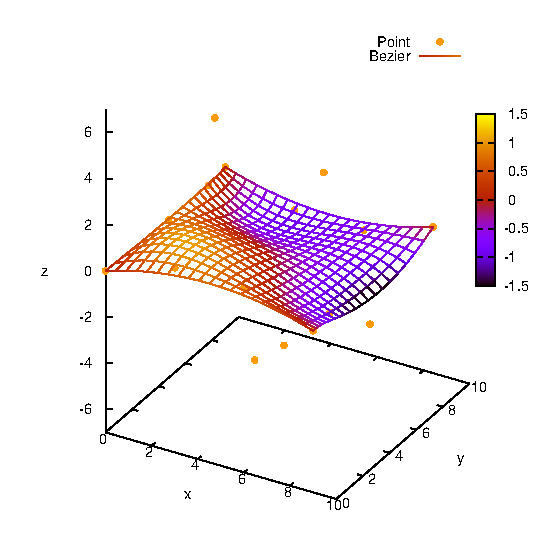
\includegraphics[width=70mm]{fig/eps/surface.eps}
  \end{center}
  \caption{パラメータ値ごとに曲面上の点}
  \label{fig:パラメータ値ごとに曲面上の点}
 \end{minipage}
 \begin{minipage}{0.5\hsize}
  \begin{center}
   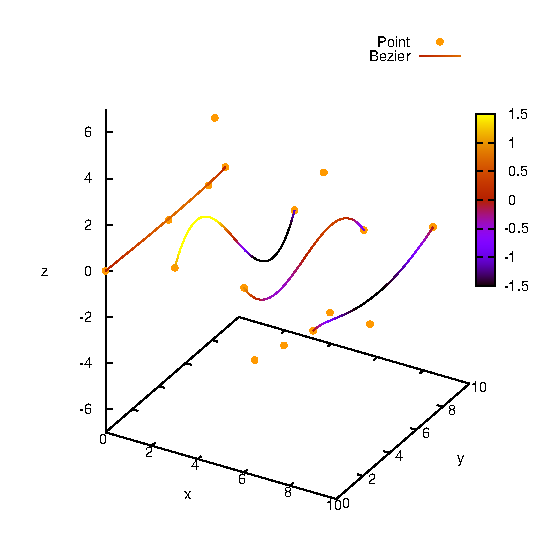
\includegraphics[width=70mm]{fig/eps/curve.eps}
  \end{center}
  \caption{曲線上の点}
  \label{fig:曲線上の点}
 \end{minipage}
\end{figure}

\begin{figure}[b]
  \centering
  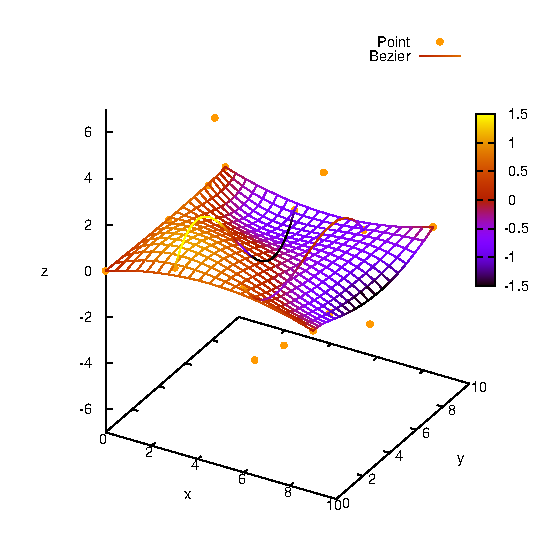
\includegraphics[width=110mm]{fig/eps/curve_surface.eps}
  \caption{ベジエ曲面と曲線を同時にプロットしたときの様子}
  \label{fig:ベジエ曲面と曲線を同時にプロットしたときの様子}
\end{figure}


\end{document}